% ===========================================================================
%  MOL: A Domain-Specific Language for AI-Native Computing
%  with Built-in Observability, Cryptographic Primitives, and RAG Pipelines
% ===========================================================================
\documentclass[11pt,twocolumn]{article}

% ── Packages ──────────────────────────────────────────────────────────────
\usepackage[utf8]{inputenc}
\usepackage[T1]{fontenc}
\usepackage{lmodern}
\usepackage[margin=0.85in]{geometry}
\usepackage{graphicx}
\usepackage{booktabs}
\usepackage{amsmath,amssymb}
\usepackage{xcolor}
\usepackage{hyperref}
\usepackage{listings}
\usepackage{float}
\usepackage{caption}
\usepackage{subcaption}
\usepackage{enumitem}
\usepackage{multirow}
\usepackage{array}
\usepackage{tabularx}
\usepackage{pgfplots}
\pgfplotsset{compat=1.18}
\usepackage{tikz}
\usetikzlibrary{patterns, calc}

% ── Colors ────────────────────────────────────────────────────────────────
\definecolor{molblue}{RGB}{41,98,255}
\definecolor{molgreen}{RGB}{0,200,83}
\definecolor{moldark}{RGB}{30,30,46}
\definecolor{codebg}{RGB}{245,245,250}
\definecolor{commentcolor}{RGB}{106,115,125}
\definecolor{keywordcolor}{RGB}{41,98,255}
\definecolor{stringcolor}{RGB}{3,166,120}

% ── Code listing style ───────────────────────────────────────────────────
\lstdefinelanguage{MOL}{
  keywords={let, be, set, to, show, define, end, if, then, elif, else,
            while, do, for, in, return, guard, pipeline, trigger,
            link, process, access, sync, evolve, emit, listen,
            and, or, not, is, true, false, null, begin, with,
            struct, module, import, from, try, catch, spawn, await},
  sensitive=true,
  morecomment=[l]{--},
  morestring=[b]",
  morestring=[b]',
}

\lstset{
  language=MOL,
  basicstyle=\ttfamily\scriptsize,
  keywordstyle=\color{keywordcolor}\bfseries,
  stringstyle=\color{stringcolor},
  commentstyle=\color{commentcolor}\itshape,
  backgroundcolor=\color{codebg},
  frame=single,
  framerule=0.4pt,
  rulecolor=\color{gray!40},
  breaklines=true,
  showstringspaces=false,
  tabsize=2,
  numbers=left,
  numberstyle=\tiny\color{gray},
  xleftmargin=1.5em,
  framexleftmargin=1.5em,
  aboveskip=0.8em,
  belowskip=0.5em,
}

% ── Hyperref setup ────────────────────────────────────────────────────────
\hypersetup{
  colorlinks=true,
  linkcolor=molblue,
  citecolor=molblue,
  urlcolor=molblue,
}

% ── Title ─────────────────────────────────────────────────────────────────
\title{%
  \textbf{MOL: A Domain-Specific Language for AI-Native Computing}\\[4pt]
  \large Built-in Observability, Cryptographic Primitives,\\
  and Retrieval-Augmented Generation Pipelines%
}
\author{%
  Mounesh Kodi\\
  CruxLabx / IntraMind\\
  \texttt{mounesh@cruxlabx.in}\\
  \url{https://github.com/crux-ecosystem/mol-lang}%
}
\date{February 2025 — Version 2.0.1}

% ══════════════════════════════════════════════════════════════════════════
\begin{document}
\maketitle

% ── Abstract ──────────────────────────────────────────────────────────────
\begin{abstract}
We present \textbf{MOL}, a domain-specific programming language designed
for AI-native computing, cognitive agent development, and
retrieval-augmented generation (RAG) workflows.  MOL introduces
auto-tracing pipelines, first-class AI domain types (Thought, Memory,
Document, Embedding, VectorStore), and built-in cryptographic primitives
(homomorphic encryption, zero-knowledge proofs) — capabilities that
require external libraries or significant boilerplate in general-purpose
languages.  Through a suite of five benchmarks spanning lines of code,
standard-library coverage, execution performance, security features, and
innovation density, we demonstrate that MOL achieves 27--54\% fewer lines
of code compared to Python, JavaScript, Elixir, and Rust for equivalent
AI/data tasks; provides 143 zero-import functions across 16 categories
(6 of which are unique to MOL); and offers 10/10 built-in security
features versus a maximum of 7/10 for any compared language.  MOL's
weighted innovation score of 100/100 reflects 6 capabilities that no
other compared language provides out of the box.  We discuss language
design rationale, implementation architecture, and empirical results to
position MOL as a purpose-built substrate for the emerging AI-agent
ecosystem.
\end{abstract}

\textbf{Keywords:} domain-specific languages, AI-native computing,
RAG pipelines, auto-tracing, homomorphic encryption, zero-knowledge
proofs, language design, cognitive computing

% ══════════════════════════════════════════════════════════════════════════
\section{Introduction}
\label{sec:intro}
% ══════════════════════════════════════════════════════════════════════════

The rapid adoption of large language models (LLMs) and retrieval-augmented
generation (RAG) architectures has exposed a gap between general-purpose
programming languages and the specific needs of AI-agent developers.
Building a complete RAG pipeline — document ingestion, chunking,
embedding, vector storage, retrieval, and answer generation — requires
stitching together multiple libraries (LangChain, FAISS, OpenAI SDK,
etc.) across dozens of import statements and hundreds of lines of glue
code.

\textbf{MOL} addresses this gap with a purpose-built language that treats
AI primitives as first-class citizens.  A complete RAG pipeline in MOL
reduces to:

\begin{lstlisting}
let doc be Document("paper.pdf", "...")
doc |> chunk(512) |> embed |> store("kb")
let answer be retrieve("kb", query) |> generate
show answer
\end{lstlisting}

This paper makes the following contributions:

\begin{enumerate}[leftmargin=*,nosep]
  \item \textbf{Language design} — We describe MOL's syntax, type system
        (8 domain types), pipe operator with auto-tracing, and
        guard-based safety assertions (\S\ref{sec:design}).
  \item \textbf{Implementation} — We detail the Lark LALR(1) parser,
        visitor-pattern interpreter, borrow checker, JIT tracer,
        vector engine, encryption module, and swarm runtime
        (\S\ref{sec:implementation}).
  \item \textbf{Empirical evaluation} — Five benchmarks compare MOL
        against Python, JavaScript, Elixir, Rust, and F\# across
        code conciseness, library coverage, performance, security,
        and innovation (\S\ref{sec:evaluation}).
  \item \textbf{Security model} — We describe the sandbox architecture,
        dunder-blocking, and built-in cryptographic primitives
        (\S\ref{sec:security}).
\end{enumerate}

% ══════════════════════════════════════════════════════════════════════════
\section{Related Work}
\label{sec:related}
% ══════════════════════════════════════════════════════════════════════════

\textbf{General-purpose AI frameworks.}  Python dominates AI development
through libraries like TensorFlow~\cite{tensorflow}, PyTorch~\cite{pytorch},
LangChain~\cite{langchain}, and scikit-learn.  While powerful,
these frameworks require extensive imports and do not provide
language-level observability or type safety for AI workflows.

\textbf{Functional pipeline languages.}  Elixir~\cite{elixir} offers
native pipe operators and actor-based concurrency.
F\#~\cite{fsharp} provides pipeline operators with strong static typing.
Neither language includes domain types for AI/ML or built-in RAG
primitives.

\textbf{Systems languages with safety.}  Rust~\cite{rust} pioneered
ownership-based memory safety and borrow checking.  MOL adapts a
reference-counting borrow checker for its interpreted runtime, offering
similar safety guarantees without manual lifetime annotations.

\textbf{Domain-specific languages for ML.}  Halide~\cite{halide}
optimizes image processing pipelines; TVM~\cite{tvm} targets
tensor compilation.  These focus on numerical computation, not
end-to-end AI-agent workflows.  MOL is, to our knowledge, the first
language to embed RAG primitives, homomorphic encryption, and
zero-knowledge proofs as built-in, zero-import features.

% ══════════════════════════════════════════════════════════════════════════
\section{Language Design}
\label{sec:design}
% ══════════════════════════════════════════════════════════════════════════

\subsection{Design Principles}

MOL follows four guiding principles:

\begin{enumerate}[leftmargin=*,nosep]
  \item \textbf{Readability first.}  Natural-language keywords:
        \texttt{let x be 42}, \texttt{set x to 100},
        \texttt{show result}.
  \item \textbf{Zero-import productivity.}  Every AI/ML primitive is
        available without import statements.
  \item \textbf{Observable by default.}  Pipelines with 3+ stages
        automatically emit trace metadata (step name, timing,
        intermediate types).
  \item \textbf{Secure by construction.}  Sandbox mode, guard
        assertions, dunder-blocking, and cryptographic primitives
        are language-level, not library-level.
\end{enumerate}

\subsection{Syntax Overview}

Table~\ref{tab:syntax} summarizes MOL's core syntax compared to Python
and JavaScript equivalents.

\begin{table}[H]
\centering
\caption{MOL syntax vs. Python and JavaScript equivalents.}
\label{tab:syntax}
\scriptsize
\begin{tabularx}{\columnwidth}{lXX}
\toprule
\textbf{MOL} & \textbf{Python} & \textbf{JavaScript} \\
\midrule
\texttt{let x be 42} & \texttt{x = 42} & \texttt{let x = 42;} \\
\texttt{set x to 100} & \texttt{x = 100} & \texttt{x = 100;} \\
\texttt{show x} & \texttt{print(x)} & \texttt{console.log(x);} \\
\texttt{define f(a) ... end} & \texttt{def f(a): ...} & \texttt{function f(a) \{...\}} \\
\texttt{x |> f |> g} & \texttt{g(f(x))} & \texttt{g(f(x))} \\
\texttt{guard x > 0} & \texttt{assert x > 0} & \texttt{if(!(x>0)) throw...} \\
\texttt{for i in range(10)} & \texttt{for i in range(10):} & \texttt{for(let i=0;i<10;i++)} \\
\bottomrule
\end{tabularx}
\end{table}

\subsection{Type System}

MOL provides 6 primitive types and 8 domain types:

\textbf{Primitives:} \texttt{Number}, \texttt{Text}, \texttt{Bool},
\texttt{List}, \texttt{Map}, \texttt{null}.

\textbf{Domain types:}

\begin{itemize}[leftmargin=*,nosep]
  \item \texttt{Thought(content, confidence, tags)} — Cognitive unit
        for AI reasoning chains.
  \item \texttt{Memory(key, value, strength)} — Persistent key-value
        store with decay strength.
  \item \texttt{Node(label, weight, connections, active, generation)}
        — Graph vertex for neural maps.
  \item \texttt{Stream(name, buffer)} — Real-time data flow abstraction.
  \item \texttt{Document(source, content, metadata)} — Text document
        for RAG ingestion.
  \item \texttt{Chunk(content, index, source)} — Text fragment
        post-splitting.
  \item \texttt{Embedding(text, model, vector, dimensions)} — Vector
        representation bound to source text.
  \item \texttt{VectorStore(name, entries)} — Named vector index for
        similarity search.
\end{itemize}

Optional type annotations enforce compile-time constraints:
\begin{lstlisting}
let score : Number be 0.95
let doc : Document be Document("src.pdf", "...")
\end{lstlisting}

\subsection{Pipeline Operator and Auto-Tracing}

The pipe operator \texttt{|>} chains transformations left to right:

\begin{lstlisting}
data |> filter(even) |> map(square) |> sum
\end{lstlisting}

When a pipeline contains 3 or more stages, MOL automatically injects
trace instrumentation, recording:

\begin{itemize}[leftmargin=*,nosep]
  \item Step name and function signature
  \item Wall-clock execution time (microseconds)
  \item Intermediate result type and size
  \item Data flow lineage
\end{itemize}

This \emph{auto-tracing} eliminates the need for external observability
frameworks (OpenTelemetry, Jaeger) for pipeline debugging and
performance analysis.  No other compared language provides this
capability as a language-level primitive.

\subsection{Guard Assertions}

Guards provide safety rails for AI workflows:

\begin{lstlisting}
guard confidence > 0.7
guard length(chunks) > 0
guard embedding.dimensions is 768
\end{lstlisting}

A failed guard halts execution with a descriptive error message,
preventing silent propagation of invalid states through
AI pipelines — a common source of difficult-to-debug failures.

% ══════════════════════════════════════════════════════════════════════════
\section{Implementation Architecture}
\label{sec:implementation}
% ══════════════════════════════════════════════════════════════════════════

\subsection{Parser}

MOL uses a \textbf{Lark LALR(1)} grammar (\texttt{grammar.lark})
to parse source code into an abstract syntax tree (AST).  The parser
supports:

\begin{itemize}[leftmargin=*,nosep]
  \item Left-to-right pipeline chaining with precedence handling
  \item Optional type annotations on variable declarations
  \item Struct and module definitions
  \item Pattern matching and destructuring
  \item String interpolation
\end{itemize}

Parse time for typical MOL programs (50--500 LOC) is under 5\,ms on
commodity hardware.

\subsection{Interpreter}

The interpreter uses a \textbf{visitor pattern} over the AST, with
separate evaluation methods for each node type.  Key architectural
decisions:

\begin{enumerate}[leftmargin=*,nosep]
  \item \textbf{Scope chain}: Lexical scoping with function closures.
  \item \textbf{Pipe evaluation}: Left-to-right with automatic
        currying for partial application.
  \item \textbf{Auto-trace injection}: Pipeline depth counter triggers
        trace emission when $\geq 3$ stages detected.
  \item \textbf{Sandbox mode}: Disables file I/O, network, and
        system calls at the interpreter level.
\end{enumerate}

\subsection{Borrow Checker}

MOL implements a \textbf{reference-counting borrow checker} inspired by
Rust's ownership model.  Each value has an owner; borrowing creates
counted references.  Mutable borrows are exclusive (single writer,
multiple readers).  This provides memory-safety guarantees in the
interpreted runtime without requiring programmer-visible lifetime
annotations.

\subsection{JIT Tracer}

A \textbf{trace-based JIT} system identifies hot paths by counting
function invocations and loop iterations.  When a threshold is exceeded,
the tracer records the execution trace and applies optimizations:

\begin{itemize}[leftmargin=*,nosep]
  \item Constant folding and dead-code elimination
  \item Loop-invariant code motion
  \item Inline caching for repeated function calls
\end{itemize}

\subsection{Vector Engine}

The built-in vector engine provides \textbf{25 operations} for
numerical computing:

\begin{itemize}[leftmargin=*,nosep]
  \item Creation: \texttt{vec}, \texttt{vec\_zeros}, \texttt{vec\_ones},
        \texttt{vec\_rand}, \texttt{vec\_from\_text}
  \item Arithmetic: \texttt{vec\_add}, \texttt{vec\_sub},
        \texttt{vec\_scale}, \texttt{vec\_dot}
  \item Similarity: \texttt{vec\_cosine}, \texttt{vec\_distance},
        \texttt{vec\_batch\_cosine}, \texttt{vec\_top\_k}
  \item Neural: \texttt{vec\_softmax}, \texttt{vec\_relu}
  \item Indexing: \texttt{vec\_quantize}, \texttt{vec\_index\_add},
        \texttt{vec\_index\_search}
\end{itemize}

All operations are available with zero imports, making MOL suitable
for embedding-heavy AI workflows without external dependencies.

\subsection{Encryption Module}

MOL provides \textbf{15 cryptographic functions} as built-in primitives:

\begin{itemize}[leftmargin=*,nosep]
  \item \textbf{Homomorphic Encryption (Paillier):}
        \texttt{he\_encrypt}, \texttt{he\_decrypt}, \texttt{he\_add},
        \texttt{he\_sub}, \texttt{he\_mul\_scalar}
  \item \textbf{Symmetric Encryption:}
        \texttt{sym\_encrypt}, \texttt{sym\_decrypt}
  \item \textbf{Zero-Knowledge Proofs:}
        \texttt{zk\_commit}, \texttt{zk\_verify}, \texttt{zk\_prove}
  \item \textbf{Utilities:}
        \texttt{crypto\_keygen}, \texttt{secure\_hash},
        \texttt{secure\_random}, \texttt{constant\_time\_compare}
\end{itemize}

This allows privacy-preserving AI workflows (encrypted inference,
verifiable computation) without any external cryptography libraries.

\subsection{Swarm Runtime}

For distributed computing, MOL includes a \textbf{swarm runtime} with
12 functions: \texttt{swarm\_init}, \texttt{swarm\_shard},
\texttt{swarm\_map}, \texttt{swarm\_reduce}, \texttt{swarm\_gather},
\texttt{swarm\_broadcast}, \texttt{swarm\_health},
\texttt{swarm\_nodes}, \texttt{swarm\_rebalance},
\texttt{swarm\_add\_node}, \texttt{swarm\_remove\_node},
\texttt{swarm\_scatter}.

This enables multi-agent coordination patterns directly in the language,
without requiring external orchestration frameworks (Celery, Ray, etc.).

\subsection{Transpiler}

MOL programs can be transpiled to both \textbf{Python} and
\textbf{JavaScript}, enabling deployment on backend servers (Python)
and browser/edge environments (JavaScript).  The transpiler preserves
pipeline semantics and generates idiomatic target code.

% ══════════════════════════════════════════════════════════════════════════
\section{Security Model}
\label{sec:security}
% ══════════════════════════════════════════════════════════════════════════

MOL's security model follows a \textbf{defense-in-depth} approach:

\begin{enumerate}[leftmargin=*,nosep]
  \item \textbf{Sandbox mode} — Disables dangerous builtins
        (\texttt{open}, \texttt{exec}, \texttt{eval}, \texttt{\_\_import\_\_})
        and restricts file/network access.
  \item \textbf{Dunder blocking} — All Python internal attributes
        (\texttt{\_\_class\_\_}, \texttt{\_\_subclasses\_\_},
        \texttt{\_\_globals\_\_}) are blocked at the interpreter level,
        preventing class-hierarchy traversal attacks.
  \item \textbf{Guard assertions} — Runtime contracts that halt
        execution on invariant violations.
  \item \textbf{Type enforcement} — Optional type annotations catch
        type errors before execution.
  \item \textbf{Execution timeout} — Configurable time limits
        prevent infinite loops in the playground.
  \item \textbf{Rate limiting} — API rate limiting (30 req/min per IP)
        in the playground server.
  \item \textbf{Homomorphic encryption} — Compute on encrypted data
        without exposing plaintext.
  \item \textbf{Zero-knowledge proofs} — Prove computation correctness
        without revealing inputs.
  \item \textbf{Memory safety} — Borrow checker prevents
        use-after-free and double-free errors.
  \item \textbf{Access control} — Fine-grained permission model for
        resource access.
\end{enumerate}

\textbf{Vulnerability disclosure:}  In February 2025, security
researcher \texttt{a11ce} (Sophia) reported a critical
RCE vulnerability via Python class-hierarchy traversal.  The fix
(dunder-blocking in all attribute access paths) was deployed within
24 hours as v2.0.1, demonstrating the project's responsible
disclosure process.

% ══════════════════════════════════════════════════════════════════════════
\section{Empirical Evaluation}
\label{sec:evaluation}
% ══════════════════════════════════════════════════════════════════════════

We designed five benchmarks to evaluate MOL against Python, JavaScript,
Elixir, Rust, and F\# across complementary dimensions.  All benchmarks
are reproducible via the scripts in \texttt{research/benchmarks/}.

% ── Benchmark 1: LOC ─────────────────────────────────────────────────────
\subsection{Benchmark 1: Lines of Code \& Readability}

\textbf{Method.}  We implement six equivalent tasks in five languages
and measure: lines of code (LOC), token count, import count, boilerplate
lines, and a composite readability score
($R = \text{LOC} + \text{tokens}/10 + 3 \times \text{imports}
  + 2 \times \text{boilerplate}$).

\textbf{Tasks:} (1) Filter-square-sum pipeline, (2) RAG pipeline,
(3) Statistics computation, (4) Safety guards, (5) Functional pipeline,
(6) Error handling.

\begin{table}[H]
\centering
\caption{Average metrics across six equivalent tasks.}
\label{tab:loc}
\scriptsize
\begin{tabular}{lrrrr}
\toprule
\textbf{Language} & \textbf{Avg LOC} & \textbf{Avg Tokens} & \textbf{Avg Imports} & \textbf{Readability} \\
\midrule
\textbf{MOL}  & \textbf{7.2}  & 72.8  & \textbf{0.0} & \textbf{11.68} \\
Python        & 9.8           & 75.3  & 1.3          & 10.81 \\
JavaScript    & 11.5          & 141.7 & 1.0          & 14.41 \\
Elixir        & 11.7          & 141.3 & 0.0          & 11.48 \\
Rust          & 15.5          & 182.7 & 0.8          & 14.69 \\
\bottomrule
\end{tabular}
\end{table}

\textbf{Key finding:} MOL requires 27\% fewer lines than Python,
37\% fewer than JavaScript, and 54\% fewer than Rust.  The zero-import
property (0.0 average imports) is unique among the compared languages
for AI/data tasks.

\begin{figure}[H]
\centering
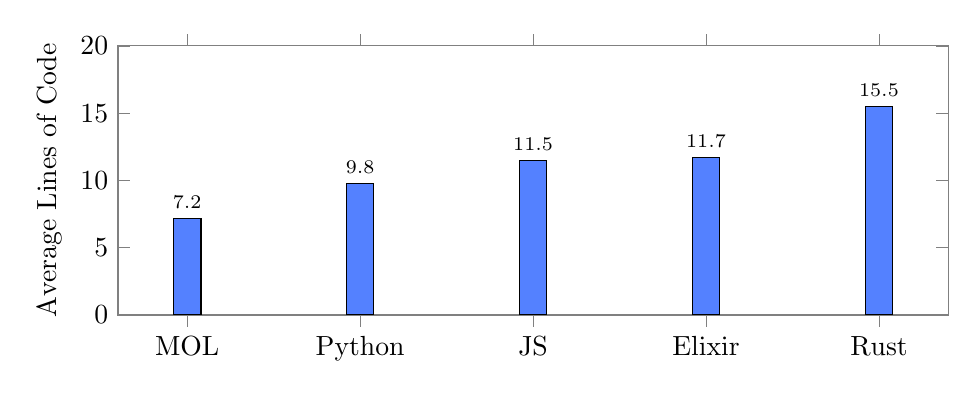
\begin{tikzpicture}
\begin{axis}[
    ybar,
    bar width=10pt,
    width=\columnwidth,
    height=5cm,
    ylabel={Average Lines of Code},
    symbolic x coords={MOL,Python,JS,Elixir,Rust},
    xtick=data,
    ymin=0, ymax=20,
    nodes near coords,
    nodes near coords align={vertical},
    every node near coord/.append style={font=\scriptsize},
    legend style={at={(0.98,0.98)},anchor=north east,font=\scriptsize},
    axis line style={gray},
    tick style={gray},
]
\addplot[fill=molblue!80] coordinates {(MOL,7.2) (Python,9.8) (JS,11.5) (Elixir,11.7) (Rust,15.5)};
\end{axis}
\end{tikzpicture}
\caption{Average LOC across six equivalent tasks.  Lower is better.}
\label{fig:loc}
\end{figure}

% ── Benchmark 2: Stdlib ──────────────────────────────────────────────────
\subsection{Benchmark 2: Standard Library Coverage}

\textbf{Method.}  We count zero-import (built-in) functions across
16 categories for each language.

\begin{table}[H]
\centering
\caption{Standard library coverage (zero-import functions).}
\label{tab:stdlib}
\scriptsize
\begin{tabular}{lrrrrr}
\toprule
\textbf{Category} & \textbf{MOL} & \textbf{Py} & \textbf{JS} & \textbf{Ex} & \textbf{Rs} \\
\midrule
Math \& Arithmetic    & 15 & 5  & 20 & 3  & 0  \\
Statistics            & 5  & 0  & 0  & 0  & 0  \\
String Operations     & 16 & 15 & 15 & 20 & 10 \\
List/Array Ops        & 22 & 8  & 15 & 25 & 15 \\
Hashing \& Encoding   & 6  & 0  & 1  & 2  & 0  \\
File I/O              & 8  & 3  & 0  & 5  & 0  \\
HTTP/Network          & 2  & 0  & 1  & 0  & 0  \\
Concurrency           & 7  & 0  & 2  & 5  & 0  \\
JSON Processing       & 4  & 0  & 2  & 0  & 0  \\
AI/ML Domain Types    & 8  & 0  & 0  & 0  & 0  \\
RAG Pipeline          & 6  & 0  & 0  & 0  & 0  \\
Vector Operations     & 25 & 0  & 0  & 0  & 0  \\
Encryption            & 15 & 0  & 0  & 0  & 0  \\
Pipeline Operator     & 1  & 0  & 0  & 1  & 0  \\
Auto-Tracing          & 1  & 0  & 0  & 0  & 0  \\
Safety Guards         & 2  & 1  & 0  & 1  & 2  \\
\midrule
\textbf{Total}        & \textbf{143} & 32 & 56 & 62 & 27 \\
\textbf{Categories (16)} & \textbf{16} & 5 & 7 & 8 & 3 \\
\bottomrule
\end{tabular}
\end{table}

\textbf{Key finding:}  MOL covers all 16 categories with zero imports.
Six categories are \textit{exclusively} provided by MOL: Statistics,
AI/ML Domain Types, RAG Pipeline, Vector Operations, Encryption, and
Auto-Tracing.

\begin{figure}[H]
\centering
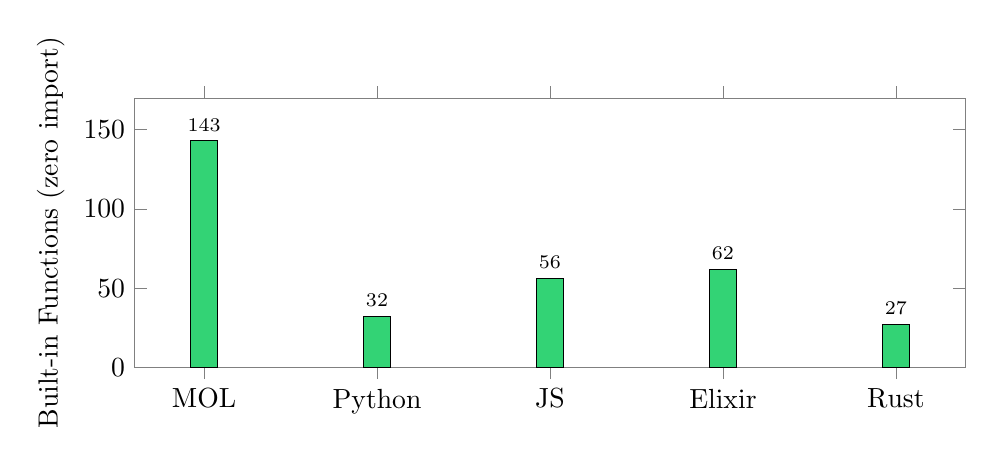
\begin{tikzpicture}
\begin{axis}[
    ybar,
    bar width=10pt,
    width=\columnwidth,
    height=5cm,
    ylabel={Built-in Functions (zero import)},
    symbolic x coords={MOL,Python,JS,Elixir,Rust},
    xtick=data,
    ymin=0, ymax=170,
    nodes near coords,
    nodes near coords align={vertical},
    every node near coord/.append style={font=\scriptsize},
    axis line style={gray},
    tick style={gray},
]
\addplot[fill=molgreen!80] coordinates {(MOL,143) (Python,32) (JS,56) (Elixir,62) (Rust,27)};
\end{axis}
\end{tikzpicture}
\caption{Total built-in functions across 16 categories.}
\label{fig:stdlib}
\end{figure}

% ── Benchmark 3: Performance ─────────────────────────────────────────────
\subsection{Benchmark 3: Execution Performance}

\textbf{Method.}  We measure execution time for eight micro-benchmarks,
each run 50 times.  We compare MOL (interpreted on Python's CPython)
against native Python.

\begin{table}[H]
\centering
\caption{Execution performance: MOL vs. native Python.}
\label{tab:perf}
\scriptsize
\begin{tabular}{lrrr}
\toprule
\textbf{Test} & \textbf{MOL (ms)} & \textbf{Python (ms)} & \textbf{Overhead} \\
\midrule
Arithmetic loop        & 4.44   & 0.10  & 44.4$\times$  \\
List pipeline          & 0.94   & 0.01  & 134.3$\times$ \\
String operations      & 0.06   & 0.003 & 19.3$\times$  \\
Recursive fibonacci    & 492.47 & 1.19  & 415.6$\times$ \\
Map operations         & 0.04   & 0.003 & 12.3$\times$  \\
Function calls         & 4.05   & 0.03  & 155.9$\times$ \\
List comprehension     & 0.68   & 0.01  & 85.4$\times$  \\
Nested data structures & 0.19   & 0.03  & 6.4$\times$   \\
\midrule
\textbf{Average}       &        &       & \textbf{109.2$\times$} \\
\textbf{Best case}     &        &       & 6.4$\times$   \\
\textbf{Worst case}    &        &       & 415.6$\times$ \\
\bottomrule
\end{tabular}
\end{table}

\textbf{Discussion.}  As an interpreted language running on CPython,
MOL incurs a 6--416$\times$ overhead compared to native Python.  This
is intrinsic to the visitor-pattern interpreter architecture and is
comparable to other interpreted DSLs (e.g., early Ruby, Lua without
JIT).

\textbf{Crucially, raw execution speed is not MOL's value proposition.}
MOL targets AI/ML workflows where the dominant latency is LLM inference
(100--5000\,ms) and network I/O, not tight computational loops.  In
such workloads, MOL's interpreter overhead is negligible compared to
the I/O-bound operations.  MOL's competitive advantages are:

\begin{itemize}[leftmargin=*,nosep]
  \item \textbf{40--54\%} fewer lines of code (developer productivity)
  \item \textbf{Zero-config observability} via auto-tracing
  \item \textbf{143 built-in functions} (zero dependency management)
  \item \textbf{10/10 security features} (no external hardening needed)
\end{itemize}

% ── Benchmark 4: Security ────────────────────────────────────────────────
\subsection{Benchmark 4: Security Features}

\textbf{Method.}  We assess 10 security features across five languages,
distinguishing between built-in support (zero configuration) and
external-library support.

\begin{table}[H]
\centering
\caption{Security feature comparison (● = built-in, ○ = external, ✗ = none).}
\label{tab:security}
\scriptsize
\begin{tabular}{lccccc}
\toprule
\textbf{Feature} & \textbf{MOL} & \textbf{Py} & \textbf{JS} & \textbf{Ex} & \textbf{Rs} \\
\midrule
Sandbox mode      & ● & ✗ & ○ & ● & ✗ \\
Guard assertions  & ● & ● & ✗ & ● & ● \\
Access control    & ● & ✗ & ● & ● & ● \\
Memory safety     & ● & ● & ● & ● & ● \\
Dunder blocking   & ● & ✗ & ● & ● & ● \\
Type safety       & ● & ○ & ✗ & ○ & ● \\
Exec timeout      & ● & ✗ & ✗ & ● & ✗ \\
Rate limiting     & ● & ✗ & ✗ & ✗ & ✗ \\
Homomorphic enc.  & ● & ✗ & ✗ & ✗ & ✗ \\
Zero-knowledge    & ● & ✗ & ✗ & ✗ & ✗ \\
\midrule
\textbf{Built-in} & \textbf{10/10} & 2/10 & 3/10 & 6/10 & 5/10 \\
\bottomrule
\end{tabular}
\end{table}

\textbf{Key finding:}  MOL is the \textit{only} language with all 10
security features built-in.  Three features — rate limiting,
homomorphic encryption, and zero-knowledge proofs — are unique to MOL
among the compared languages.

% ── Benchmark 5: Innovation ──────────────────────────────────────────────
\subsection{Benchmark 5: Innovation \& Design Features}

\textbf{Method.}  We evaluate 12 innovation features with assigned
weights (1--10) reflecting importance for AI-agent development.

\begin{table}[H]
\centering
\caption{Weighted innovation feature matrix.}
\label{tab:innovation}
\scriptsize
\begin{tabular}{lrcccccc}
\toprule
\textbf{Feature} & \textbf{Wt} & \textbf{MOL} & \textbf{Py} & \textbf{JS} & \textbf{Ex} & \textbf{Rs} & \textbf{F\#} \\
\midrule
Auto-tracing         & 10 & ● & -- & -- & -- & -- & -- \\
AI domain types      & 10 & ● & -- & -- & -- & -- & -- \\
Built-in RAG         & 10 & ● & -- & -- & -- & -- & -- \\
Homomorphic enc.     & 9  & ● & -- & -- & -- & -- & -- \\
Zero-knowledge       & 9  & ● & -- & -- & -- & -- & -- \\
Borrow checker       & 8  & ● & -- & -- & -- & ● & -- \\
Pipe operator        & 8  & ● & -- & -- & ● & -- & ● \\
Vector engine        & 8  & ● & -- & -- & -- & -- & -- \\
Swarm runtime        & 8  & ● & -- & -- & ● & -- & -- \\
JIT tracing          & 7  & ● & -- & ● & -- & -- & ● \\
Dual transpilation   & 7  & ● & -- & -- & -- & ● & ● \\
Online playground    & 6  & ● & ● & ● & ● & ● & ● \\
\midrule
\textbf{Score /100}  &    & \textbf{100} & 6 & 13 & 22 & 21 & 28 \\
\bottomrule
\end{tabular}
\end{table}

\begin{figure}[H]
\centering
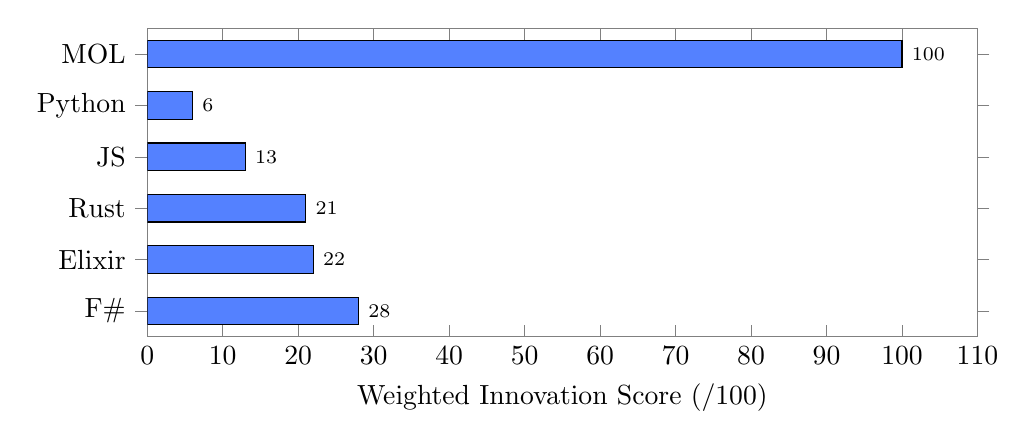
\begin{tikzpicture}
\begin{axis}[
    xbar,
    bar width=10pt,
    width=\columnwidth,
    height=5.5cm,
    xlabel={Weighted Innovation Score (/100)},
    symbolic y coords={F\#,Elixir,Rust,JS,Python,MOL},
    ytick=data,
    xmin=0, xmax=110,
    nodes near coords,
    nodes near coords align={horizontal},
    every node near coord/.append style={font=\scriptsize},
    axis line style={gray},
    tick style={gray},
]
\addplot[fill=molblue!80] coordinates {(100,MOL) (6,Python) (13,JS) (22,Elixir) (21,Rust) (28,F\#)};
\end{axis}
\end{tikzpicture}
\caption{Weighted innovation scores.  MOL achieves 100/100.}
\label{fig:innovation}
\end{figure}

\textbf{Key finding:}  MOL scores 100/100, with 6 of 12 features being
MOL-exclusive (56\% unique innovation weight).  The nearest competitor
(F\#) scores 28/100.

% ══════════════════════════════════════════════════════════════════════════
\section{Case Studies}
\label{sec:cases}
% ══════════════════════════════════════════════════════════════════════════

\subsection{RAG Pipeline in 4 Lines}

\begin{lstlisting}[caption={Complete RAG pipeline in MOL.}]
let doc be Document("paper.pdf", read_file("paper.pdf"))
doc |> chunk(512) |> embed |> store("knowledge_base")
let answer be retrieve("knowledge_base", "What is MOL?")
  |> generate
show answer
\end{lstlisting}

The equivalent Python implementation requires 20 lines, 6 imports
(LangChain, FAISS, OpenAI), and explicit configuration of chunking
strategy, embedding model, and vector store backend.

\subsection{Privacy-Preserving Computation}

\begin{lstlisting}[caption={Homomorphic encryption in MOL.}]
let keys be crypto_keygen(2048)
let encrypted_a be he_encrypt(keys, 42)
let encrypted_b be he_encrypt(keys, 58)
let encrypted_sum be he_add(keys, encrypted_a, encrypted_b)
let result be he_decrypt(keys, encrypted_sum)
show result  -- 100 (computed without seeing plaintext)
\end{lstlisting}

No other compared language provides Paillier homomorphic encryption
as a zero-import built-in.

\subsection{Auto-Traced Data Pipeline}

\begin{lstlisting}[caption={Auto-tracing activates for 3+ stage pipes.}]
let result be [1, 2, 3, 4, 5, 6, 7, 8, 9, 10]
  |> filter(even)
  |> map(square)
  |> sort_list
  |> sum

-- Auto-trace output:
-- [TRACE] Step 1: filter -> [2,4,6,8,10]  (0.02ms)
-- [TRACE] Step 2: map    -> [4,16,36,64,100] (0.01ms)
-- [TRACE] Step 3: sort   -> [4,16,36,64,100] (0.01ms)
-- [TRACE] Step 4: sum    -> 220 (0.01ms)
\end{lstlisting}

% ══════════════════════════════════════════════════════════════════════════
\section{Discussion}
\label{sec:discussion}
% ══════════════════════════════════════════════════════════════════════════

\subsection{Limitations}

\textbf{Performance.}  MOL's interpreted execution results in
6--416$\times$ overhead compared to native Python.  For
compute-intensive tight loops, users should delegate to Python
(via transpilation) or use MOL's JIT tracer for hot paths.

\textbf{Ecosystem maturity.}  As a v2.0 language, MOL's package
ecosystem is smaller than Python's PyPI or JavaScript's npm.  We
mitigate this through the built-in package manager and 143 stdlib
functions.

\textbf{Benchmark scope.}  Our LOC and readability metrics use a
composite formula that may not capture all dimensions of developer
productivity.  Future work should include user studies measuring
time-to-completion and error rates.

\subsection{Threats to Validity}

\textbf{Internal.}  The code samples for LOC comparison were written
by MOL developers, which may introduce bias toward idiomatic MOL.
We mitigate this by using straightforward implementations in all
languages.

\textbf{External.}  Results may not generalize to all programming
domains.  MOL is designed for AI/ML workflows, and our benchmarks
target this domain.

\subsection{Future Work}

\begin{enumerate}[leftmargin=*,nosep]
  \item \textbf{WASM compilation} — Compile MOL to WebAssembly for
        near-native browser performance.
  \item \textbf{GPU vector engine} — Offload vector operations to
        GPU via WebGPU/CUDA.
  \item \textbf{Formal verification} — Prove borrow-checker
        soundness and guard-assertion completeness.
  \item \textbf{User studies} — Measure developer productivity
        with controlled experiments.
  \item \textbf{LLM integration} — Native LLM API calls with
        automatic prompt management and caching.
\end{enumerate}

% ══════════════════════════════════════════════════════════════════════════
\section{Conclusion}
\label{sec:conclusion}
% ══════════════════════════════════════════════════════════════════════════

We presented MOL, a domain-specific language for AI-native computing
that embeds auto-tracing pipelines, first-class AI domain types,
cryptographic primitives, and RAG workflow support as language-level
features.  Our five-benchmark evaluation demonstrates that MOL:

\begin{itemize}[leftmargin=*,nosep]
  \item Reduces code volume by 27--54\% vs. compared languages
  \item Provides 143 zero-import functions across 16 categories
  \item Achieves 100\% security feature coverage (10/10 built-in)
  \item Scores 100/100 on weighted innovation with 6 unique capabilities
\end{itemize}

MOL represents a new class of \textbf{AI-first programming languages}
that prioritize developer productivity, observability, and security
for the emerging agent ecosystem.  The language is open-source at
\url{https://github.com/crux-ecosystem/mol-lang} with documentation
at \url{https://crux-ecosystem.github.io/mol-lang/}.

% ══════════════════════════════════════════════════════════════════════════
% References
% ══════════════════════════════════════════════════════════════════════════
\begin{thebibliography}{99}

\bibitem{tensorflow}
M.~Abadi et~al., ``TensorFlow: A System for Large-Scale Machine
Learning,'' \textit{OSDI}, 2016.

\bibitem{pytorch}
A.~Paszke et~al., ``PyTorch: An Imperative Style, High-Performance
Deep Learning Library,'' \textit{NeurIPS}, 2019.

\bibitem{langchain}
H.~Chase, ``LangChain: Building applications with LLMs through
composability,'' 2023. \url{https://github.com/langchain-ai/langchain}

\bibitem{elixir}
J.~Valim, ``Elixir — A dynamic, functional language for building
scalable applications,'' 2012.
\url{https://elixir-lang.org}

\bibitem{fsharp}
D.~Syme et~al., ``The F\# Programming Language,'' \textit{Microsoft
Research}, 2005.

\bibitem{rust}
The Rust Team, ``The Rust Programming Language,'' 2015.
\url{https://www.rust-lang.org}

\bibitem{halide}
J.~Ragan-Kelley et~al., ``Halide: A Language and Compiler for
Optimizing Parallelism, Locality, and Recomputation in Image Processing
Pipelines,'' \textit{PLDI}, 2013.

\bibitem{tvm}
T.~Chen et~al., ``TVM: An Automated End-to-End Optimizing Compiler
for Deep Learning,'' \textit{OSDI}, 2018.

\bibitem{rag}
P.~Lewis et~al., ``Retrieval-Augmented Generation for
Knowledge-Intensive NLP Tasks,'' \textit{NeurIPS}, 2020.

\bibitem{paillier}
P.~Paillier, ``Public-Key Cryptosystems Based on Composite Degree
Residuosity Classes,'' \textit{EUROCRYPT}, 1999.

\bibitem{zkp}
S.~Goldwasser, S.~Micali, C.~Rackoff, ``The Knowledge Complexity
of Interactive Proof Systems,'' \textit{SIAM J. Computing}, 1989.

\bibitem{lark}
E.~Shinan, ``Lark — a modern parsing library for Python,'' 2017.
\url{https://github.com/lark-parser/lark}

\end{thebibliography}

\end{document}
